\section{Introduction}
\label{sec:introduction}

Monitoring plant biodiversity at scale is essential for understanding ecosystem health, tracking the effects of climate change, and informing conservation policy. Traditionally, vegetation surveys require expert botanists to visit field sites, place standardised quadrats (typically 50$\times$50\,cm sampling frames), and manually identify every plant species visible within the frame. This process is labour-intensive, difficult to scale, and constrained by the availability of trained taxonomists~\cite{joly2024overview}.

The PlantCLEF 2026 challenge~\cite{plantclef2026} seeks to automate this task by framing it as a multi-label classification problem: given a high-resolution photograph of a vegetation quadrat, predict the set of all plant species present. The challenge draws from a taxonomy of approximately 7,800 candidate species, and submissions are evaluated using a macro-averaged F1 score computed per sample and then aggregated across transects.

A central difficulty of this challenge is the \emph{domain shift} between the available training data and the target test data. The training set consists of over one million single-plant images from the PlantCLEF 2024 corpus, each depicting an individual specimen with a single species label (Figure~\ref{fig:train_grid}). In contrast, the test images are dense, complex vegetation scenes where multiple species overlap, occlude one another, and appear at varying scales and growth stages (Figure~\ref{fig:quadrats}). Models trained exclusively on isolated specimens tend to perform poorly when confronted with these multi-species scenes, as they have never encountered the visual complexity of real-world vegetation during training.

\begin{figure*}[t]
  \centering
  \resizebox{0.92\linewidth}{!}{% Training-image grid — 6 representative PlantCLEF~2024 single-plant
% images, 2 rows x 3 columns. The image filenames are content hashes
% from the PC24 distribution; no species captions are shown here
% (species are described in the host caption).
%
% Required host preamble:
%   \usepackage{graphicx}
%   \usepackage{tikz}

\begin{tikzpicture}[
  every node/.style={inner sep=0pt, outer sep=0pt},
]

\def\cellw{50mm}
\def\cellh{50mm}
\def\colsep{2mm}
\def\rowsep{3mm}

% ── Row 1 ──────────────────────────────────────────────────────────────
\node                                       (t1) at (0, 0) {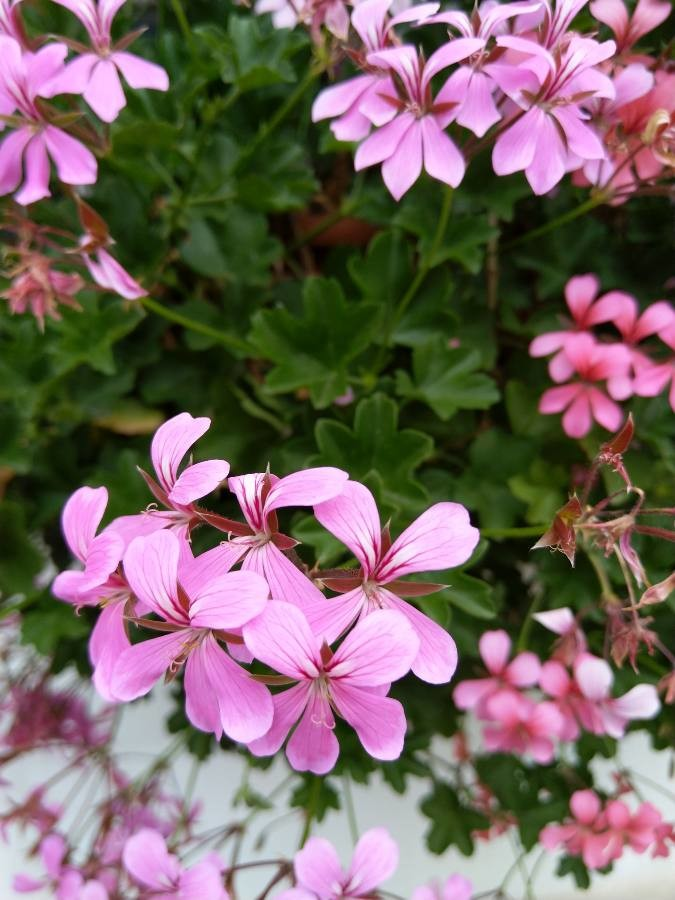
\includegraphics[width=\cellw, height=\cellh, keepaspectratio]{images/train/0b4007a0ea47ce9a04625baca25ce8b31eaafb44.jpg}};
\node[right=\colsep of t1.east, anchor=west](t2)            {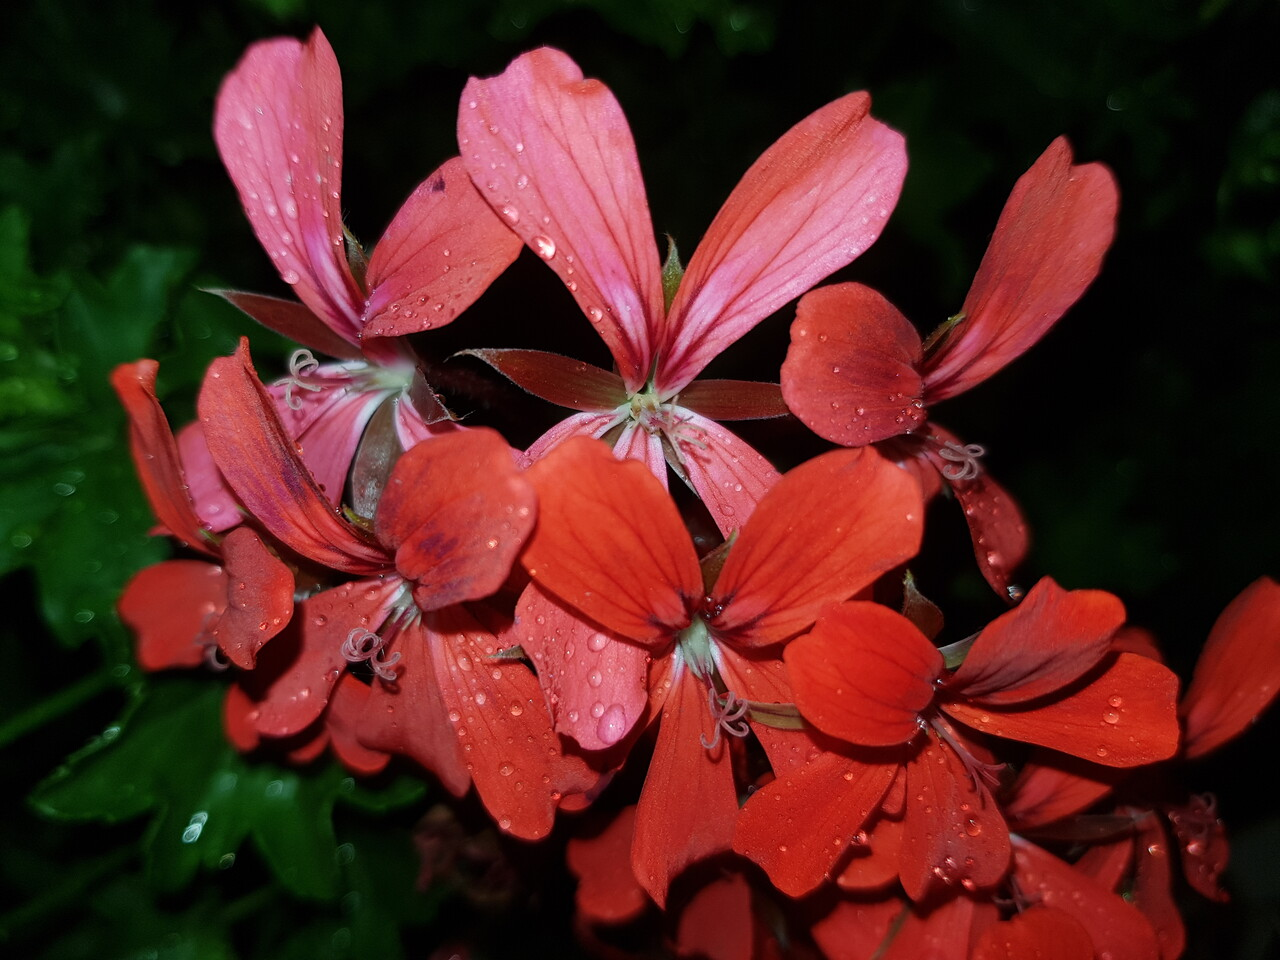
\includegraphics[width=\cellw, height=\cellh, keepaspectratio]{images/train/0b5296be0cd6e68cf46f7331edbc54ae600a0f1d.jpg}};
\node[right=\colsep of t2.east, anchor=west](t3)            {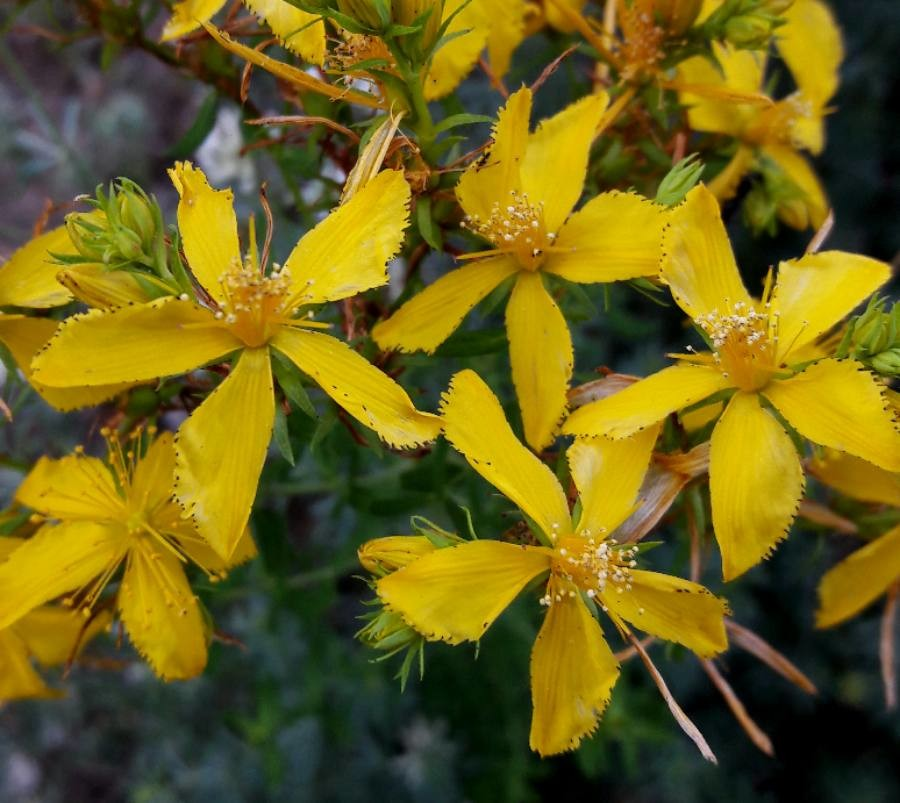
\includegraphics[width=\cellw, height=\cellh, keepaspectratio]{images/train/0c5ab5fd302458218691c7833a97688793a7466f.jpg}};

% ── Row 2 ──────────────────────────────────────────────────────────────
\node[below=\rowsep of t1.south, anchor=north]              (t4) {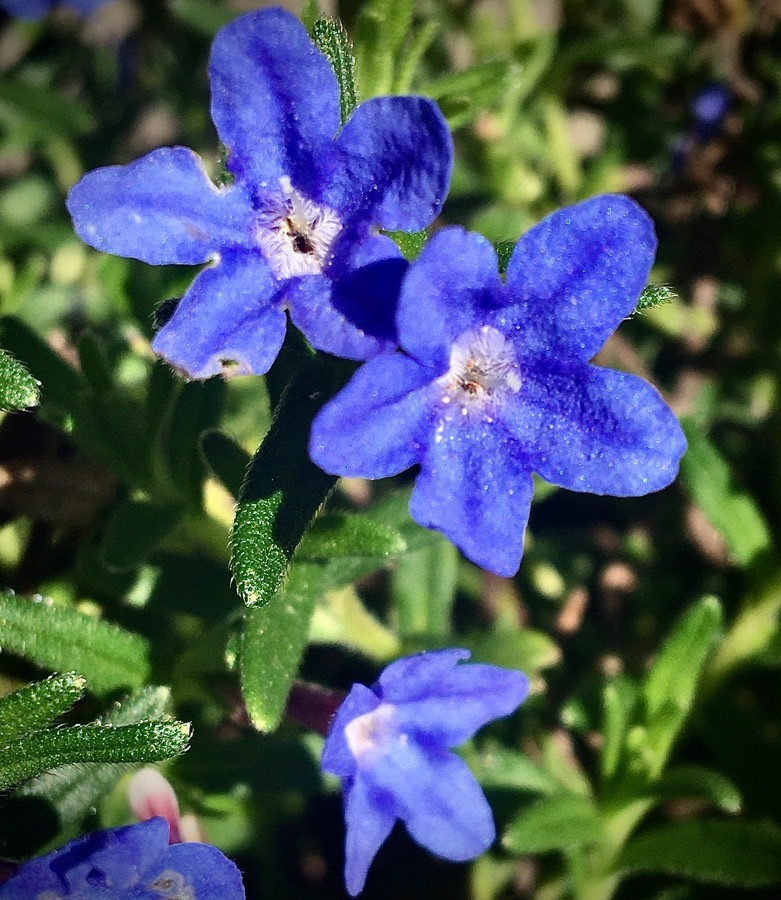
\includegraphics[width=\cellw, height=\cellh, keepaspectratio]{images/train/3f2b6248fa328d486b33b4f77f65d6b18b74c5c6.jpg}};
\node[right=\colsep of t4.east, anchor=west]                (t5) {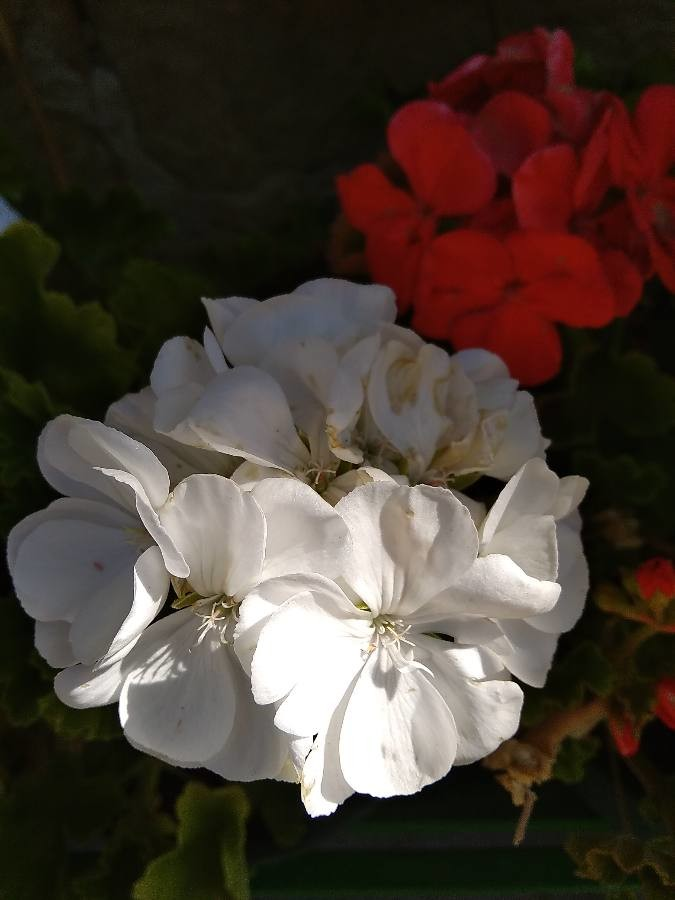
\includegraphics[width=\cellw, height=\cellh, keepaspectratio]{images/train/9cf6b7997a95b2bab8d840e70397b98dc8321106.jpg}};
\node[right=\colsep of t5.east, anchor=west]                (t6) {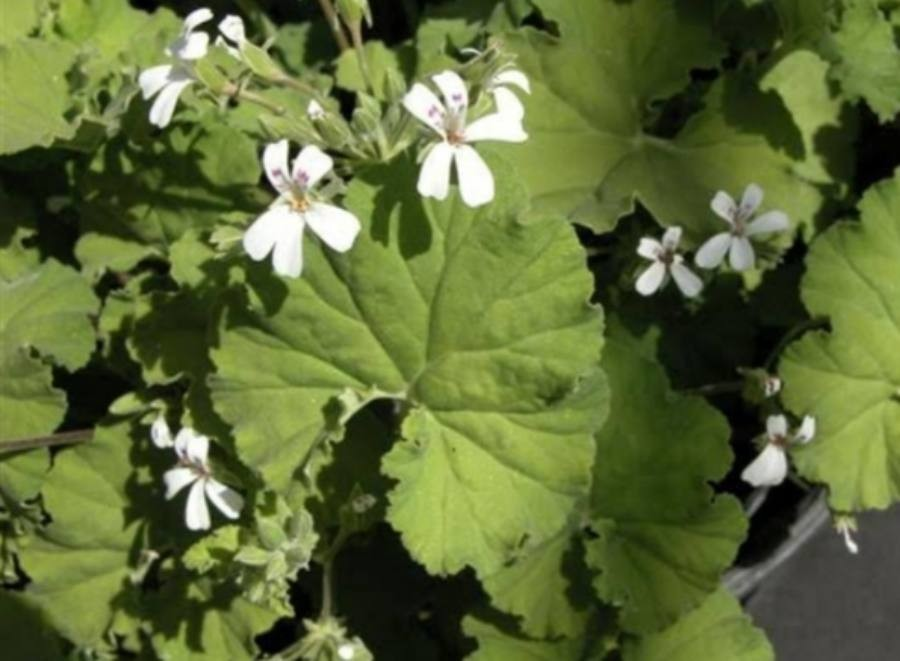
\includegraphics[width=\cellw, height=\cellh, keepaspectratio]{images/train/fe3131163544feb319ec6754b79ca33007177e95.jpg}};

\end{tikzpicture}
}
  \caption{Six representative single-plant training images from the PlantCLEF~2024 corpus. Each image carries a single species label and was contributed through the Pl@ntNet citizen-science pipeline. Shooting style is intentionally varied (close-up macro, half-body, full-plant in habitat) and lighting / background are uncontrolled.}
  \label{fig:train_grid}
\end{figure*}

\begin{figure*}[t]
  \centering
  \resizebox{0.92\linewidth}{!}{% Quadrat-grid figure — 6 representative test-set quadrats arranged 2×3.
% Each cell shows the quadrat photograph with its filename (which
% encodes the transect site + date) as a caption above.
%
% Required host preamble:
%   \usepackage{graphicx}
%   \usepackage{tikz}
%
% Images live in archive/report/images/quadrats/.

\begin{tikzpicture}[
  every node/.style={inner sep=0pt, outer sep=0pt},
  label/.style={font=\sffamily\tiny, text=black!70, align=center},
]

% Cell dimensions: 3 columns, 2 rows; ~5.4cm wide cells leaves slight gap
\def\cellw{52mm}
\def\cellh{52mm}
\def\colsep{2mm}
\def\rowsep{6mm}

% ── Row 1 ──────────────────────────────────────────────────────────────
\node[label]                              (l1) at (0,                              0)              {CBN-PdlC-A1-20130807.jpg};
\node[below=1mm of l1]                    (i1)                                                     {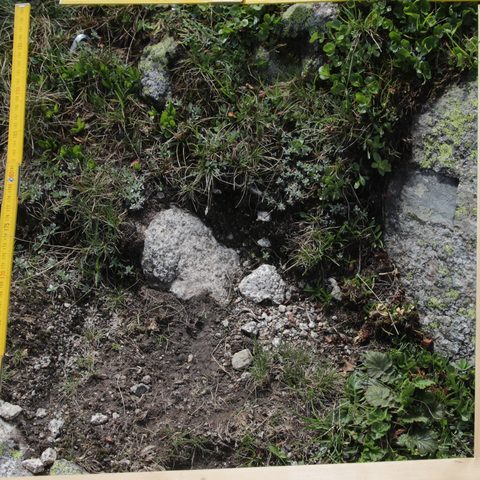
\includegraphics[width=\cellw, height=\cellh, keepaspectratio]{images/quadrats/CBN-PdlC-A1-20130807.jpg}};

\node[label, right=\colsep of l1.east, anchor=west] (l2) {CBN-Pla-A1-20130808.jpg};
\node[below=1mm of l2]                              (i2) {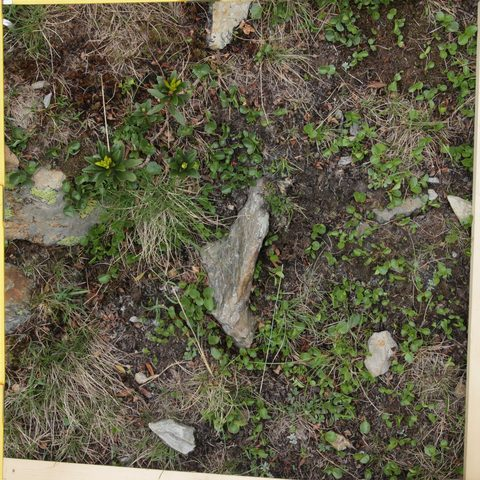
\includegraphics[width=\cellw, height=\cellh, keepaspectratio]{images/quadrats/CBN-Pla-A1-20130808.jpg}};

\node[label, right=\colsep of l2.east, anchor=west] (l3) {GUARDEN-CBNMed-10-1-16-34-20240429.jpg};
\node[below=1mm of l3]                              (i3) {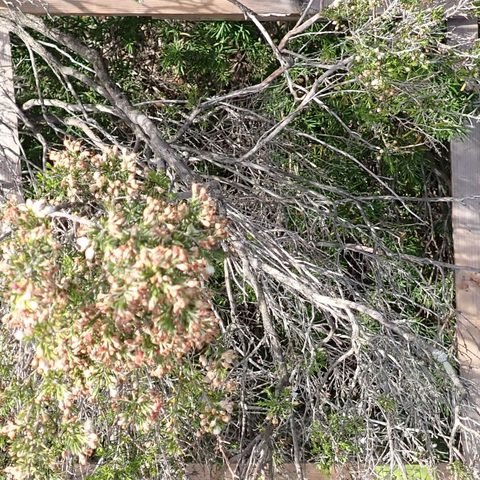
\includegraphics[width=\cellw, height=\cellh, keepaspectratio]{images/quadrats/GUARDEN-CBNMed-10-1-16-34-20240429.jpg}};

% ── Row 2 ──────────────────────────────────────────────────────────────
\node[label, below=\rowsep of i1.south] (l4) {LISAH-JAS-0-1-20220505.jpg};
\node[below=1mm of l4]                  (i4) {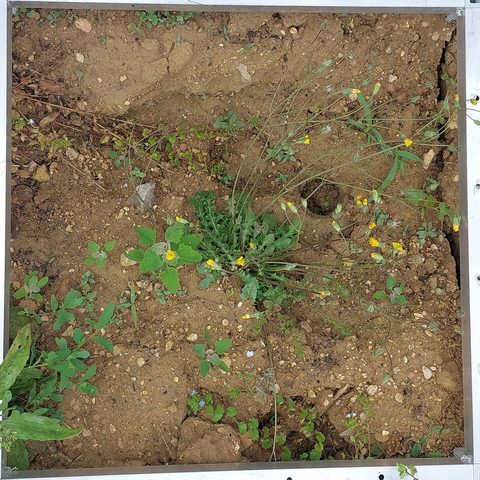
\includegraphics[width=\cellw, height=\cellh, keepaspectratio]{images/quadrats/LISAH-JAS-0-1-20220505.jpg}};

\node[label, right=\colsep of l4.east, anchor=west] (l5) {OPTMix-0108-P1-312-20231006.jpg};
\node[below=1mm of l5]                              (i5) {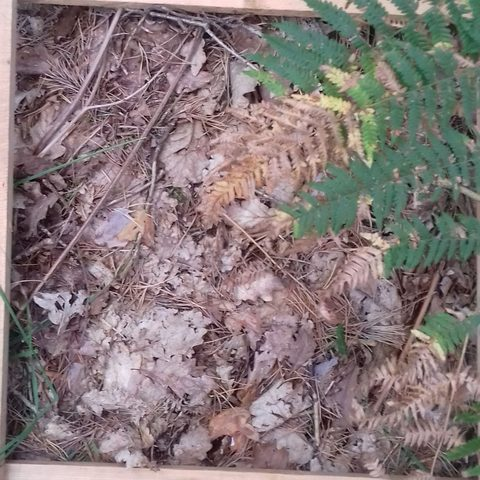
\includegraphics[width=\cellw, height=\cellh, keepaspectratio]{images/quadrats/OPTMix-0108-P1-312-20231006.jpg}};

\node[label, right=\colsep of l5.east, anchor=west] (l6) {RNNB-1-1-20230512.jpg};
\node[below=1mm of l6]                              (i6) {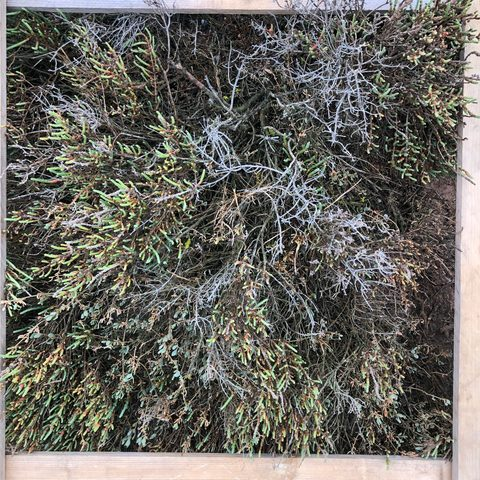
\includegraphics[width=\cellw, height=\cellh, keepaspectratio]{images/quadrats/RNNB-1-1-20230512.jpg}};

\end{tikzpicture}
}
  \caption{Six representative quadrats from the PlantCLEF 2026 test set, illustrating the breadth of within-set domain variation. Filenames (left to right): \texttt{CBN-PdlC-A1-20130807}, \texttt{CBN-Pla-A1-20130808}, \texttt{GUARDEN-CBNMed-10-1-16-34-20240429}, \texttt{LISAH-JAS-0-1-20220505}, \texttt{OPTMix-0108-P1-312-20231006}, \texttt{RNNB-1-1-20230512}. Each filename encodes the transect site and observation date. The quadrats range from dense mid-summer canopies (CBN-PdlC, RNNB) to dry shrub-mat communities (LISAH, GUARDEN) and litter-covered shoulder-season frames (OPTMix). Shooting angle, sampling-frame style (wood, tape, painted line), and illumination all vary across the corpus, compounding the single-plant\,$\to$\,multi-species domain shift seen in Figure~\ref{fig:train_grid}.}
  \label{fig:quadrats}
\end{figure*}

A second major challenge is the \emph{long-tail distribution} of the training data. While common species may have thousands of training images, rare species---which are often the most ecologically important---can have fewer than ten. Standard cross-entropy training causes models to overwhelmingly predict common classes, yielding high micro-accuracy but poor macro-F1.

In this paper, we present the system submitted by the Australian National University (ANU) team. Our approach centres on three key design decisions:

\begin{enumerate}
  \item \textbf{Partial-unfreeze BioCLIP 2.5 with taxonomic regularisation.} BioCLIP~\cite{stevens2024bioclip} is a contrastive vision-language model whose pretraining on TreeOfLife-10M aligns its feature space with the Linnaean taxonomy. Rather than fine-tuning the full backbone---which we show collapses this prior---we unfreeze only the last four transformer blocks of BioCLIP 2.5 ViT-H/14 and attach auxiliary cross-entropy heads at coarser taxonomic levels (genus and family in the deployed model; an earlier multi-task fine-tune additionally used order and class). The auxiliary losses carry small fixed weights, with coarser levels weighted progressively less, so that they primarily regularise the encoder rather than drive it.
  \item \textbf{Long-tail data rebalancing.} The PlantCLEF 2024 single-plant corpus is heavily skewed: a small number of species exceed one thousand training images while hundreds carry fewer than ten. We attack this from both ends, by augmenting the manifest with extra observations for under-represented species and by applying a per-species image cap that flattens the head of the distribution. We find that on this benchmark, more training data and a flatter species distribution dominate gains from additional unfrozen capacity.
  \item \textbf{Tile-level inference with adaptive selection.} At inference we partition each quadrat into a $4{\times}4$ grid of $448$-pixel tiles with no overlap, forward each tile through the encoder at both $224$ and $336$ pixels, and aggregate the per-tile softmax distributions by per-species mean across both the sixteen tiles and the two resolutions. Class-prior logit adjustment ($\tau{=}0.25$) is then applied. Final selection is adaptive: we emit every species whose post-adjusted probability exceeds a fixed threshold ($T{=}0.03$), with a floor of two and a ceiling of ten species per quadrat. The 224 + 336 resolution ensemble lifts the public score by $+0.007$ over the single-resolution baseline; the adaptive threshold outperforms fixed top-$k$ selection by between $0.005$ and $0.008$ Macro F1.
\end{enumerate}

The remainder of this paper is organised as follows. Section~\ref{sec:related} reviews related work on plant identification, foundation model adaptation, and multi-label classification. Section~\ref{sec:method} describes our system architecture and training procedure in detail. Section~\ref{sec:experiments} presents our experimental setup and results. Section~\ref{sec:conclusion} concludes with a discussion of limitations and directions for future work.
